\documentclass[a4paper]{article}
\usepackage{amssymb}
\usepackage{bbm}
\usepackage[normalem]{ulem}
\usepackage{graphicx}
\usepackage[colorlinks,linkcolor=blue,anchorcolor=blue,citecolor=blue,urlcolor=blue]{hyperref}
\usepackage{mciteplus}
\usepackage{etoolbox}
\usepackage{tikz}
\usetikzlibrary{shapes}

\title{Statement of Research}
\author{JinGuo Liu\\ Department of Physics, Harvard University}
\date{\today}

\newcommand{\<}{\langle}
\renewcommand{\>}{\rangle}
\newcommand{\vsigma}{\vec{\sigma}}
\setlength{\topmargin}{-10mm}
\setlength{\textwidth}{7in}
\setlength{\oddsidemargin}{-8mm}
\setlength{\textheight}{9in}
\setlength{\footskip}{1in}

\begin{document}
\fontsize{10}{13}
\selectfont
\maketitle

I am a Post-Doctoral Fellow in Mikhail Lukin's group at the department of physics at Harvard University with an interest in understanding the connection between computing and physics.
In the past decades, these two seemingly unrelated fields are more and more inter-weaved.
It brings many beautiful theories that deepened our understanding toward the nature of computing and the nature of our physical world.
For example, 
%Another example is recent advances in understanding the hardness of problems from the overlap gap properties that highly inspired from the phase transition in spin glasses.
by relating the energy consumption in computation and a quantum system with environment, researchers showed why the Landauer's principle (every irreversible bit operation dissipates an energy lower bounded by $k_bT\ln 2$ to the environment) is true from a simple quantum computational model;
by relating a universal quantum Turing machine with a local Hamiltonian, researchers show the problem of telling whether a local Hamiltonian or an initial state thermalize if is uncomputable, i.e. as hard as the famous halting problem in computer science.

The majority of my current research is also about relating computing and physics.
In the following, I will explain my past works mainly from two perspectives, one is understanding the computational hardness from the solution space properties, i.e. the energy level degeneracy and the energy landscape, another is embedding computational hard problems to a physical system.

\section{Solution space properties of hard combinatorial optimization problems}
\subsection{Current Work}
The first project that I involved in Harvard is an experiment of using variational quantum algorithms to solve the maximum independent set problem by embedding a problem instance into a Rydberg atom array Hamiltonian.
Motivated by understanding why our quantum algorithm works better than classical simulated annealing in some graph instances but not in others.
I and my collaborators created a unified framework to solve the \textit{solution space properties} of a class of hard combinatorial optimization problems. Here, the solution space property refers to a class of quantities that not only include the maximum or minimum set size, but also include the number of sets at a give size, enumeration of all sets at a give size and direct sampling of such sets when they are too large to be fit into a memory; the class of problem includes but is not limited to the independent set problem, the maximum cut problem, the vertex coloring problem, the maximal clique problem, the dominating set problem, and the satisfiability problem, among others.

The framework we created is called generic tensor network, where the word ``generic'' is from generic programming in computer science.
The relationship between counting problem and tensor network problems is known before in the field, however, these works haven't caught much attention to computational scientists since their very limited using cases.
We take a different view of a tensor network and show the algebraic structure of a tensor network is its unique advantage comparing to other algorithms such as those based on dynamic programming and branching for solving hard combinatorial optimization problems.
Instead of using the standard number types as tensor elements, we engineer tensor element types being members of a commutative semiring algebra as show in Figure \ref{fig:venn-diagram} that each relates a solution space property.
%which is highly inspired by the recent advances about random tensor network benchmarking quantum supremacy.
The real algebra is related to the counting problem, the (extended) tropical algebra is related the largest solution size(s), the polynomial algebra is related the graph polynomials, the truncated polynomial algebra is related to the degeneracy of solutions with largest or smallest several sizes, the bit string algebra is related to finding one best solution and the set algebra is related to solution enumeration.

\begin{figure}[th]
   \centering
\centerline{\begin{tikzpicture}[]
    \scriptsize
    \node[draw,fill=lime!80,fill opacity=1, text opacity=1.0,ellipse,minimum width=2cm, minimum height=1cm,inner sep=0pt] at (0, 2.5) (R) {$\mathbbm{R}$};
    \def\dx{-3};
    \node[draw,fill=teal!50,fill opacity=1, text opacity=1.0,ellipse,minimum width=5cm, minimum height=3cm,inner sep=0pt] at (\dx, 0) (PN) {\hspace{-3.5cm}Polynomial};
    \node[draw,fill=brown!75,fill opacity=1, text opacity=1.0,ellipse,minimum width=3.5cm, minimum height=1.0cm,inner sep=0pt] at (\dx, 0.7) (P1) {\hspace{-1.0cm}Largest order};
    \node[draw,fill=brown!40,fill opacity=1, text opacity=1.0,ellipse,minimum width=3.5cm, minimum height=1.0cm,inner sep=0pt] at (\dx, -0.4) (P2) {\hspace{-0.8cm}Largest 2 orders};
    \node[draw,fill=brown,fill opacity=1, text opacity=1.0,ellipse,minimum width=0.8cm, minimum height=0.3cm,inner sep=0pt] at (\dx, 1.0) (T) {};
    \node[draw,fill=brown!50,fill opacity=1, text opacity=1.0,ellipse,minimum width=0.8cm, minimum height=0.3cm,inner sep=0pt] at (\dx, -0.1) (T2) {};
    \node at (\dx, -1.2) {$\ldots$};
    \node[above = 1cm] at (T) (textT) {Tropical};
    \node[below = 2cm, left=4cm] (textT2) {Extended Tropical};
    \draw[black,-latex] (textT) -- (T);
    \draw[black,-latex] (textT2) -- (T2);

    % set and set sampler
    \node[draw,fill=yellow,fill opacity=0.5, text opacity=1.0,ellipse,minimum width=5cm, minimum height=3cm,inner sep=0pt] at (0, 0) (SN) {};
    \node[below of=1] at (SN) {Set};
    \node[draw,fill=red!70,fill opacity=0.5, text opacity=1.0,ellipse,minimum width=4cm, minimum height=1.5cm,inner sep=0pt] at (-0.5, 0) (S1) {\hspace{1.5cm}Bit string};
\end{tikzpicture}}

    \caption{The the tensor network element types used in this work and their relationships.
    The overlap between two ellipses indicates that a new algebra can be created by combining those two algebras. ``Largest order'' and ``Largest 2 orders'' mean truncating the polynomial by only keeping its largest or largest two orders.} \label{fig:venn-diagram}
\end{figure}

% the understanding we have
Our methodology deepened our understanding to the MIS experiment. We find a good indicator of the hardness, which is the degeneracy ratio.
We also find the absence of the overlap gap properties in the target problem from the configuration enumeration, which is an important feature to identify hardness of a combinatorial problem for local search based algorithms.

% benefit to open source community
I created an open source package \href{}{GraphTensorNetworks} that might benefit people in the field of computational complexity and statistic physics.
During developing this package, I also have a lot side contribution to the open source community, the \href{}{TropicalGEMM} for fast matrix multiplication (very close to the theoretical optimal speed, i.e. half the speed of floating point number), optimized \texttt{permutedims} on CUDA and \href{}{OMEinsumContractionOrders} for the state of the art contraction order optimization algorithms for random tensor networks.

\subsection{Future Work}
It would be interesting to generalize the idea of generic programming to other algorithms for property computing with certain algebraic structures such as those using the inclusion-exclusion principle or subset convolution.
To this end, it is worth mentioning the dynamic programming.
Dynamic programming is closely related to a tensor network, for example, the Viterbi algorithm for finding most probable configuration in the hidden Markov model has a nice matrix product state interpretation, and the tropical tensor network is very likely equivalent to dynamic programming in solving hard combinatorial optimization problems in certain way.
However, while having broader applications,
%e.g. the traveling sales man can be solved easily with dynamic programming but not with a tensor network to the best of our knowledge, 
dynamic programming does not have a clear algebraic interpretation for computing solution space properties beyond finding best solutions.

\section{Algorithms targeting near-term intermediate scale quantum devices}
\subsection{Current Work}

\begin{figure}
\centering
\begin{subfigure}[b]{0.25\textwidth}
\includegraphics[width=\textwidth, trim={0cm 0cm 0cm 0cm}, clip]{images/petersen.pdf}
\caption{}
\end{subfigure}\hspace{20pt}
\begin{subfigure}[b]{0.6\textwidth}
\includegraphics[width=\textwidth, trim={0cm 0cm 0cm 0cm}, clip]{images/petersen_mapped.pdf}
\caption{}
\end{subfigure}
\caption{(a) The Petersen graph and (b) its diagonal coupled unit disk grid graph embedding.}\label{fig:petersen}
\end{figure}

Reduction is an important method to.
\subsection{Future Work}

\section{Summary}
To summarize, the this point in my career, my primary interests are computational hard problems and their implication to physics.

\end{document}
